%%NEW frase
\begin{frame}{El paper en una frase}
  \begin{block}{}
    \large ¿Cómo leer un puntero compartido a un objeto con conteo de referencias \textbf{mientras otro hilo lo cambia}, sin candados, sin que nadie espere y sin gastar memoria extra?
  \end{block}
  \bigskip
  \begin{itemize}
    \item Euro-Par 2024 (LNCS 14803), Utrecht y CMU; sello \emph{Artifact Evaluated}: el código es público y lo hemos usado.
    \item Mejora el \emph{split reference count} (Folly, GCC), que solo es \emph{lock-free}: la hace \textbf{\emph{wait-free}} y más sencilla de explicar.
  \end{itemize}
\end{frame}

%%NEW rc
\begin{frame}[fragile]{Conteo de referencias y \emph{atomic shared pointer}}
  \begin{columns}[T]
    \column{0.5\textwidth}
\begin{semiverbatim}\scriptsize
auto a = std::make_shared<Libro>(); // rc = 1
\{
    auto b = a;   // copia:          rc = 2
\}                 // b se destruye:  rc = 1
a = nullptr;      // rc = 0: se libera
\end{semiverbatim}
    \begin{itemize}\small
      \item Copiar: \textbf{rc += 1}; destruir: \textbf{rc $-$= 1}.
      \item rc = 0 $\Rightarrow$ se libera \textbf{en ese momento}; con rc = 1 el dueño modifica en el sitio.
    \end{itemize}
    \column{0.46\textwidth}
    \begin{itemize}\small
      \item \textbf{Shared pointer}: puntero \emph{inmutable} con conteo; su contador ya es seguro entre hilos.
      \item \textbf{Atomic shared pointer}: celda \emph{mutable} con un shared pointer; varios hilos la leen (\texttt{load}) y la cambian (\texttt{store}).
      \item \clave{El problema nace aquí}: leer la celda y subir el contador del objeto.
    \end{itemize}
\begin{semiverbatim}\scriptsize
std::atomic<std::shared_ptr<Config>> config;
auto c = config.load();
config.store(std::make_shared<Config>(n));
\end{semiverbatim}
  \end{columns}
\end{frame}

%%NEW peso
\begin{frame}{El peso en el \emph{atomic shared pointer}}
  \begin{columns}[c]
    \column{0.55\textwidth}
    \includegraphics[width=\linewidth]{figuras/paper_fig2.pdf}
    \fuente{Fig. 2 del paper. (a) 104 + 1 + 1 = 106. (b) Tras un \texttt{load}: cartel 103, un pase nuevo, hoja sigue en 106.}
    \column{0.42\textwidth}\footnotesize
    \begin{itemize}
      \item Al crear el cartel se le da un peso $C \gg P$ y se suma $C$ a la hoja. Cada pase pesa 1.
      \item Invariante: \textbf{hoja $\ge$ peso del cartel + pases}. Por arriba es seguro; por abajo, liberaríamos con lectores dentro.
    \end{itemize}
  \end{columns}
  \medskip
  \begin{itemize}\footnotesize
    \item \textbf{Empaquetado}: el peso va en los 16 bits altos libres del puntero (x86-64 usa 48). Restar un ticket es restar $2^{48}$ a la palabra entera; la dirección no cambia:
  \end{itemize}
  \centering{\ttfamily\footnotesize 0x\textcolor{acento}{0068}\,7F3A12345670 $-$ 0x\textcolor{acento}{0001}\,000000000000 = 0x\textcolor{acento}{0067}\,7F3A12345670}
\end{frame}

%%NEW alg1
\begin{frame}{Algoritmo 1: \texttt{store} y \texttt{load}}
  \centering\includegraphics[width=0.7\linewidth]{figuras/paper_alg1.pdf}
  \fuente{Algoritmo 1 del paper.}
  \begin{columns}[T]
    \column{0.48\textwidth}\footnotesize
    \textbf{\texttt{store}}: \textbf{1.} sumar $C$ al objeto nuevo \emph{antes} de publicarlo; \textbf{2.} \texttt{swap}: poner (nuevo, $C$) y llevarse (viejo, $w$) de golpe; \textbf{3.} restar al viejo \textbf{solo} el sobrante $w$.
    \column{0.48\textwidth}\footnotesize
    \textbf{\texttt{load}}: \textbf{1.} \texttt{fetch\_and\_add}($-$\texttt{pack(null,1)}): un ticket menos y el valor anterior: \clave{una instrucción}; \textbf{2.} si quedan menos de $P$: recargar (alg.\,2); \textbf{3.} devolver un pase de peso 1.
  \end{columns}
\end{frame}

%%NEW recarga
\begin{frame}{Recargar el talonario: el punto delicado}
  \begin{columns}[T]
    \column{0.52\textwidth}\small
    Cuando un \texttt{load} deja el peso por debajo de $P$, \textbf{ese hilo} recarga: reserva $C-w$ en la hoja y sube el peso lo mismo. Hace falta un \textbf{CAS} («solo si sigue como lo vi»): el cartel pudo cambiar de libro u otro hilo pudo recargar ya.
    \begin{block}{Requisitos para ser \emph{wait-free}}
      \footnotesize\textbf{R-1}: $C \ge 2P$ (tras recargar, el peso queda $\ge 2P-(P-1) = P+1$).\\
      \textbf{R-2}: el peso solo \textbf{baja de 1 en 1} o se \textbf{fija por encima de $P$}.
    \end{block}
    \column{0.44\textwidth}
    \includegraphics[width=\linewidth]{figuras/paper_fig4.pdf}
    \fuente{Fig. 4 del paper: peso de un cartel en el tiempo; la línea es $P$.}
  \end{columns}
  \medskip\small
  Si el CAS falla y el peso \textbf{subió}, alguien ya recargó: \clave{salida temprana}. Quien mete el talonario en la zona roja, lo saca; si otro se adelanta, se va.
\end{frame}

%%NEW alg2
\begin{frame}{Algoritmo 2: \texttt{increase\_weight}}
  \centering\includegraphics[width=0.7\linewidth]{figuras/paper_alg2.pdf}
  \fuente{Algoritmo 2 del paper.}
  \begin{columns}[T]
    \column{0.55\textwidth}\footnotesize
    \textbf{1.} reservar $C-w$ en la hoja \textbf{antes} del CAS; \textbf{2.} CAS: si el cartel sigue en (ptr, actual), sumar $C-w$ y terminar; \textbf{3.} otro puntero o \textbf{peso mayor}: devolver la reserva y salir; \textbf{4.} peso menor: reintentar.
    \column{0.41\textwidth}\footnotesize
    Los pesos esperados forman una cadena \textbf{estrictamente decreciente} entre $P-1$ y 0: \clave{como mucho $P$ intentos}.
  \end{columns}
\end{frame}

%%NEW demo2
\begin{frame}{Demo 2: un simulador encuentra los fallos de cada variante}
  \centering
  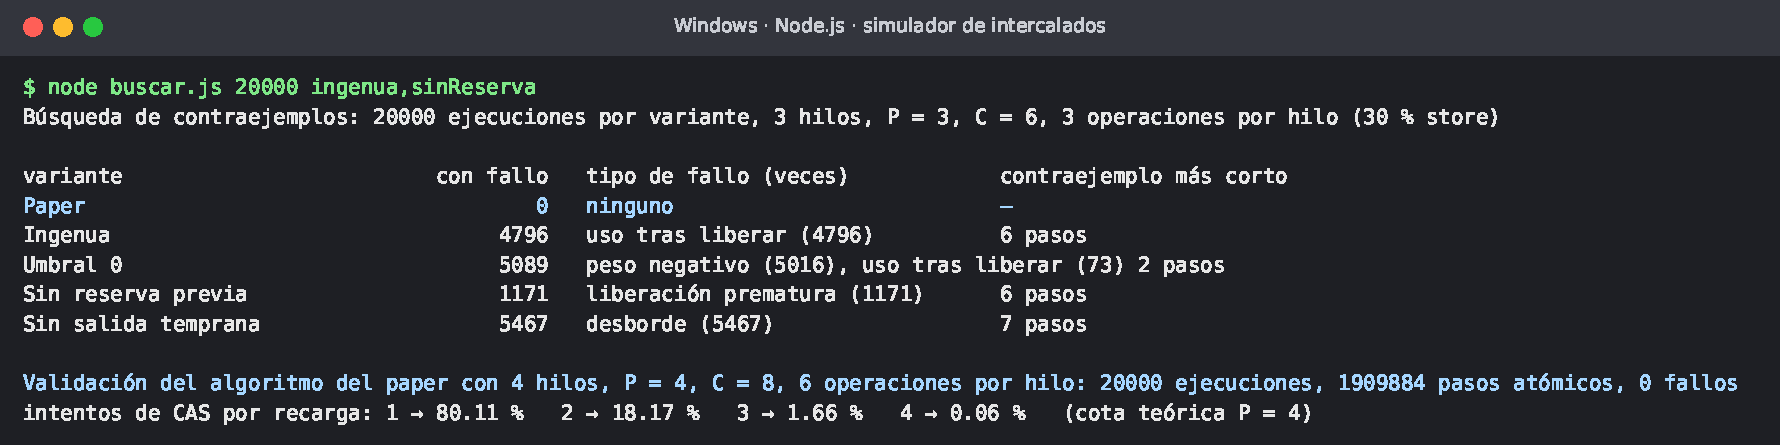
\includegraphics[width=0.98\linewidth]{graficos/captura_simulador.pdf}
  \begin{itemize}\footnotesize\raggedright
    \item Simulador de intercalados (paso atómico a paso atómico) que comprueba los invariantes tras cada paso, 20\,000 ejecuciones por variante. \textbf{Paper: 0 fallos}; cada variante rota falla en 2 a 7 pasos.
    \item Ejemplo («sin reserva»): Carla hace \texttt{load} y le toca recargar; Beto hace \texttt{swap} y resta toda la reserva: el libro se libera \textbf{con un lector dentro}.
  \end{itemize}
\end{frame}

%%NEW coste
\begin{frame}{Coste y extensiones}
  \begin{columns}[T]
    \column{0.52\textwidth}\footnotesize
    \begin{itemize}
      \item El bucle CAS solo repite si \textbf{otro} hilo bajó el peso: cadena $w_0 > w_1 > \dots \ge 0$ con $w_0 \le P-1$ $\Rightarrow$ como mucho $P$ intentos.
      \item \texttt{load}: normalmente una instrucción; \textbf{$O(P)$ solo en el peor caso} ($P$ = hilos que usan esa variable). Con $C = 2^{19}$, $P = 2^{16}$ hay $\approx$ 458\,752 lecturas entre recargas.
      \item Extensiones: \texttt{null} (el peso da la vuelta, sin recargar), punteros débiles (misma técnica) y \emph{aliasing} (dos punteros en 128 bits).
    \end{itemize}
    \column{0.44\textwidth}
    \renewcommand{\arraystretch}{1.15}\footnotesize
    \begin{tabular}{@{}p{2.1cm}p{1.9cm}l@{}}
      \toprule
      Operación & Coste & Garantía\\
      \midrule
      \texttt{store}, \texttt{swap} & $O(1)$ & \emph{wait-free}\\
      \texttt{load} & 1 instr.; $O(P)$ peor & \emph{wait-free}\\
      compare-and-swap & sin cota & \emph{lock-free}\\
      \texttt{load} \emph{aliased} & sin cota & \emph{lock-free}\\
      \bottomrule
    \end{tabular}
    \par\smallskip{\scriptsize El CAS es \emph{lock-free}: cualquier lectura cambia los tickets y hace fallar al escritor.}
  \end{columns}
\end{frame}

%%NEW exper
\begin{frame}{Experimentos del paper}
  \begin{columns}[c]
    \column{0.5\textwidth}\footnotesize
    \begin{itemize}
      \item $C = 2^{19}$, $P = 2^{16}$. Rendimiento: 144 hilos; latencia: 56 hilos.
      \item Banco: \textbf{pila concurrente} ($n$ pilas, $u$\,\% de actualizaciones). Rivales: Libstdc++ (candados), Williams y Folly (\emph{split refcount}), Anderson (\emph{hazard pointers}).
      \item Con 1 hilo, \textbf{Ours} es la más rápida; gana a los que no usan memoria extra (con 1 pila y 144 hilos, $\approx$7× Williams y $\approx$20× Folly). Frente a Anderson depende de la contención: pierde con una sola pila.
      \item \texttt{load}, $p = 56$ (mediana): \textbf{Ours 1,14\us} · Anderson 2,58\us · Folly 11,6\us · Libstdc++ 99,7\us.
    \end{itemize}
    \column{0.46\textwidth}
    \includegraphics[width=\linewidth]{figuras/paper_fig5.pdf}
    \fuente{Fig. 5 del paper: millones de operaciones por segundo frente a hilos.}
  \end{columns}
\end{frame}

%%NEW rend
\begin{frame}{Pruebas en local (2): rendimiento con el código de los autores}
  \centering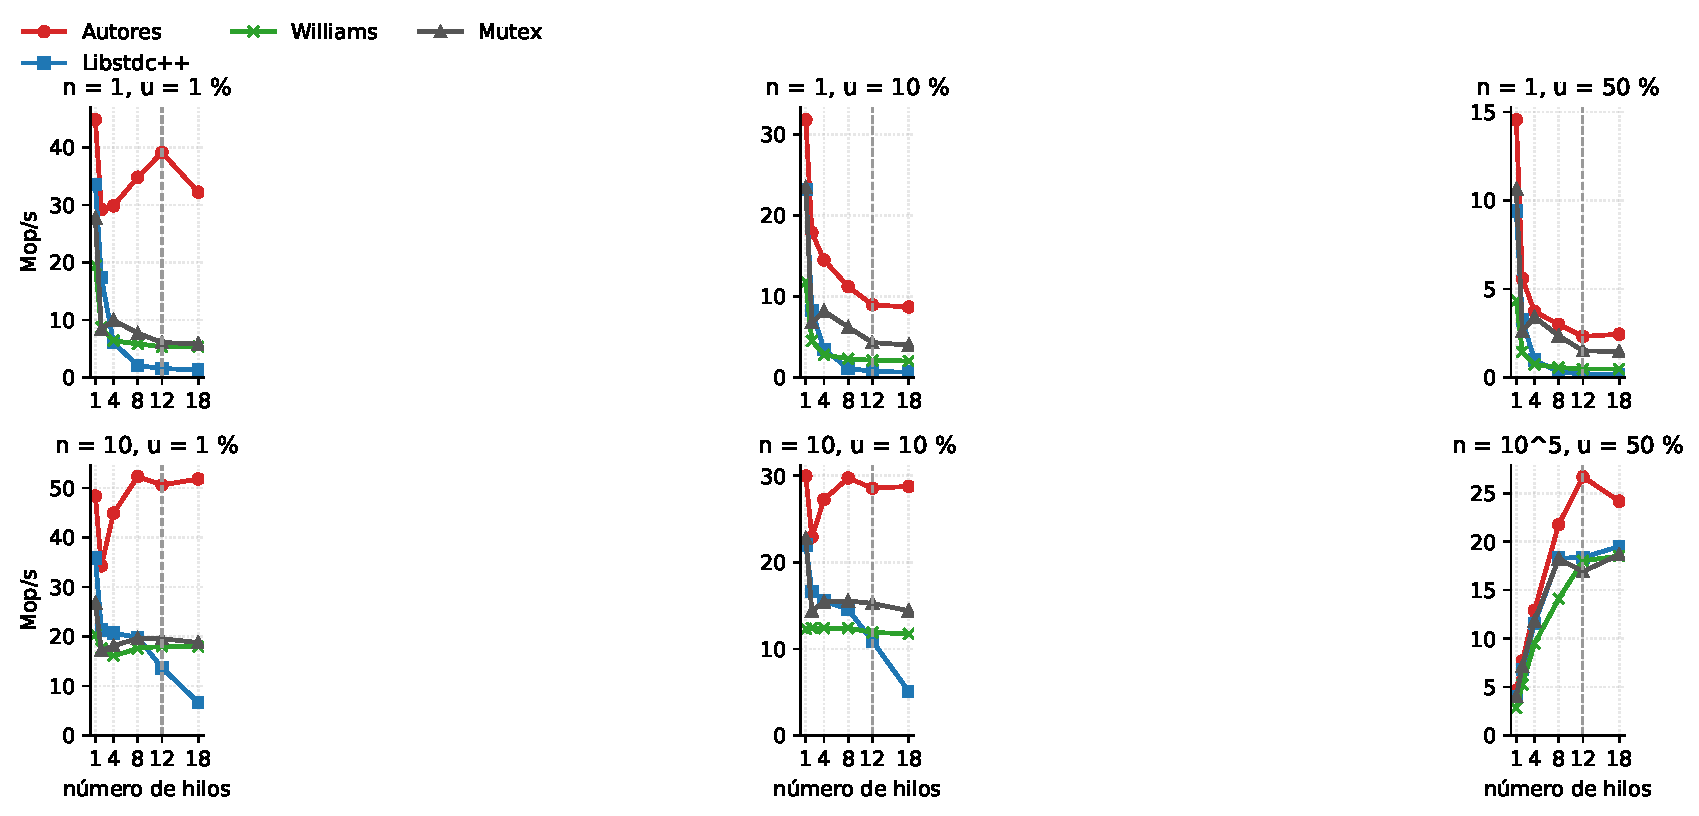
\includegraphics[width=0.74\linewidth]{graficos/local_rendimiento.pdf}
  \fuente{Mini-Fig. 5 (12 hilos): Autores, \texttt{atomic<shared\_ptr>} de GCC 13 (Libstdc++) y \texttt{std::mutex}. $n=1,u=1$: 34,3 · 2,2 · 6,4 Mop/s. Con $n=1,u=50$ el mutex gana (2,9 frente a 2,2): el CAS es \emph{lock-free}. Con 1 hilo, Autores es la más rápida. Tendencias, no cifras absolutas.}
\end{frame}

%%NEW lat
\begin{frame}{Pruebas en local (3): latencia con 12 hilos}
  \centering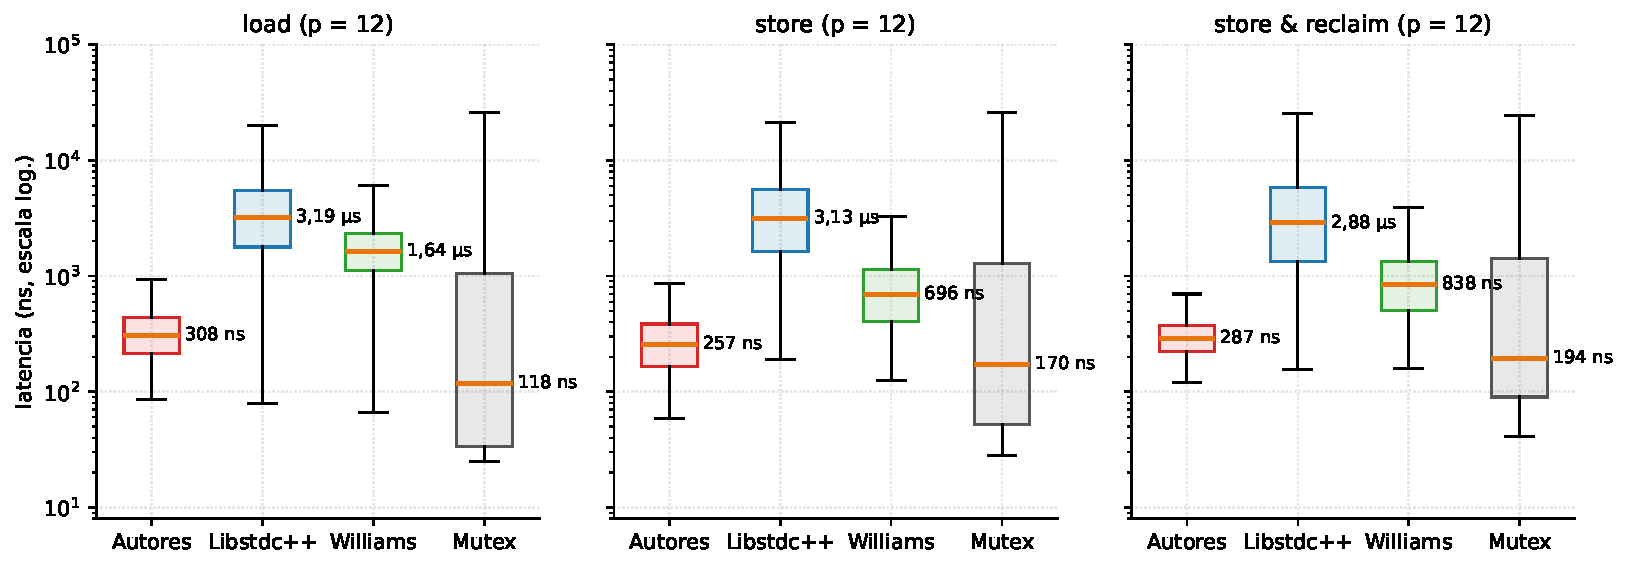
\includegraphics[width=0.72\linewidth]{graficos/local_latencia.pdf}
  \fuente{Mini-Fig. 6: 1 hilo mide y 11 hacen \texttt{store}; 100\,000 muestras. \texttt{load} (mediana / p99): Autores 269 ns / 0,83\us · Libstdc++ 3,06\us{} / 16\us · Mutex 61 ns / \textbf{27,6\us}. La mediana engaña; la cola delata a quien espera.}
\end{frame}
